\section{Basic Operations}
In the world of linear algebra, basic operations form the cornerstone of mathematical manipulations applied to our objects (scalar, vectors and matrices). These operations serve as fundamental tools for analyzing and transforming these mathematical entities, unlocking insights across various disciplines.

\subsection{Transposition}

In linear algebra, transposition refers to the operation of switching the rows and columns of a mathematical object. This operation is commonly applied to matrices, and geometrically can be interpreted as reflecting the matrix over its main diagonal.

\subsubsection{Matrix Transposition}

For a given matrix $A_{m,n} \in \mathbb F^{m \times n}$, the transpose, denoted as $A_{m,n}^T$, is obtained by swapping its rows with columns. Mathematically, each $a_{i,j}$ in $A_{m,n}$, would be mapped into $a_{ji}$. In other words, the element in the $i$-th row and $j$-th column of $A_{m,n}^T$ is the same as the element in the $j$-th row and $i$-th column of $A_{m,n}$.

So $A_{m,n}^T = A_{n,m}'$.
\\

\textbf{Example:}

Consider the following matrix:
\[
A = \begin{bmatrix}
    1 & 2 & 3 \\
    4 & 5 & 6 \\
    7 & 8 & 9 \\
\end{bmatrix}
\]

The transpose of matrix $A$ is:
\[
A^T = \begin{bmatrix}
    1 & 4 & 7 \\
    2 & 5 & 8 \\
    3 & 6 & 9 \\
\end{bmatrix}
\]

\subsubsection{Properties:}

\begin{itemize}
    \item $(A^T)^T = A$: Transposing a matrix twice results in the original matrix.
    \item $(cA)^T = cA^T$: Transposing a scaled matrix is equivalent to scaling the transpose.
    \item $(A + B)^T = A^T + B^T$: Transposing the sum of two matrices is equivalent to the sum of their transposes.
    % Product properties (A * B)^T = B^T * A^T
\end{itemize}

These properties are fundamental in various mathematical applications, including linear algebra and optimization.

% Symmetric matrix
% Antisymmetric matrix

\subsection{Addition}
In linear algebra, the sum of two objects is a fundamental operation that combines their respective components.
We are very familiar with the common sum of scalars:

$$
a + b = c,
$$
but what happens when we need to apply the sum to objects of dimension greater than 0?
\\

Vector sum, for example is defined as follow. 
\\

Let 
$$
\vec{v} = \begin{bmatrix} v_1 \\ v_2 \\ \vdots \\ v_n \end{bmatrix}, \quad \vec{w} = \begin{bmatrix} w_1 \\ w_2 \\ \vdots \\ w_n \end{bmatrix}
$$
be two vectors in \(\mathbb{F}^n\). 
    The sum of two vectors \(\vec{v}\) and \(\vec{w}\), denoted as \(\vec{v} + \vec{w}\), is defined component-wise:
    
\[ \vec{v} + \vec{w} = \begin{bmatrix} v_1 + w_1 \\ v_2 + w_2 \\ \vdots \\ v_n + w_n \end{bmatrix} \]

Geometrically, vector addition corresponds to placing the initial point of the second vector at the terminal point of the first vector and connecting the initial point of the first vector to the terminal point of the second vector (as shown in Figure \ref{fig:vector-sum-1}).
\\
\begin{figure}[h]
    \centering
    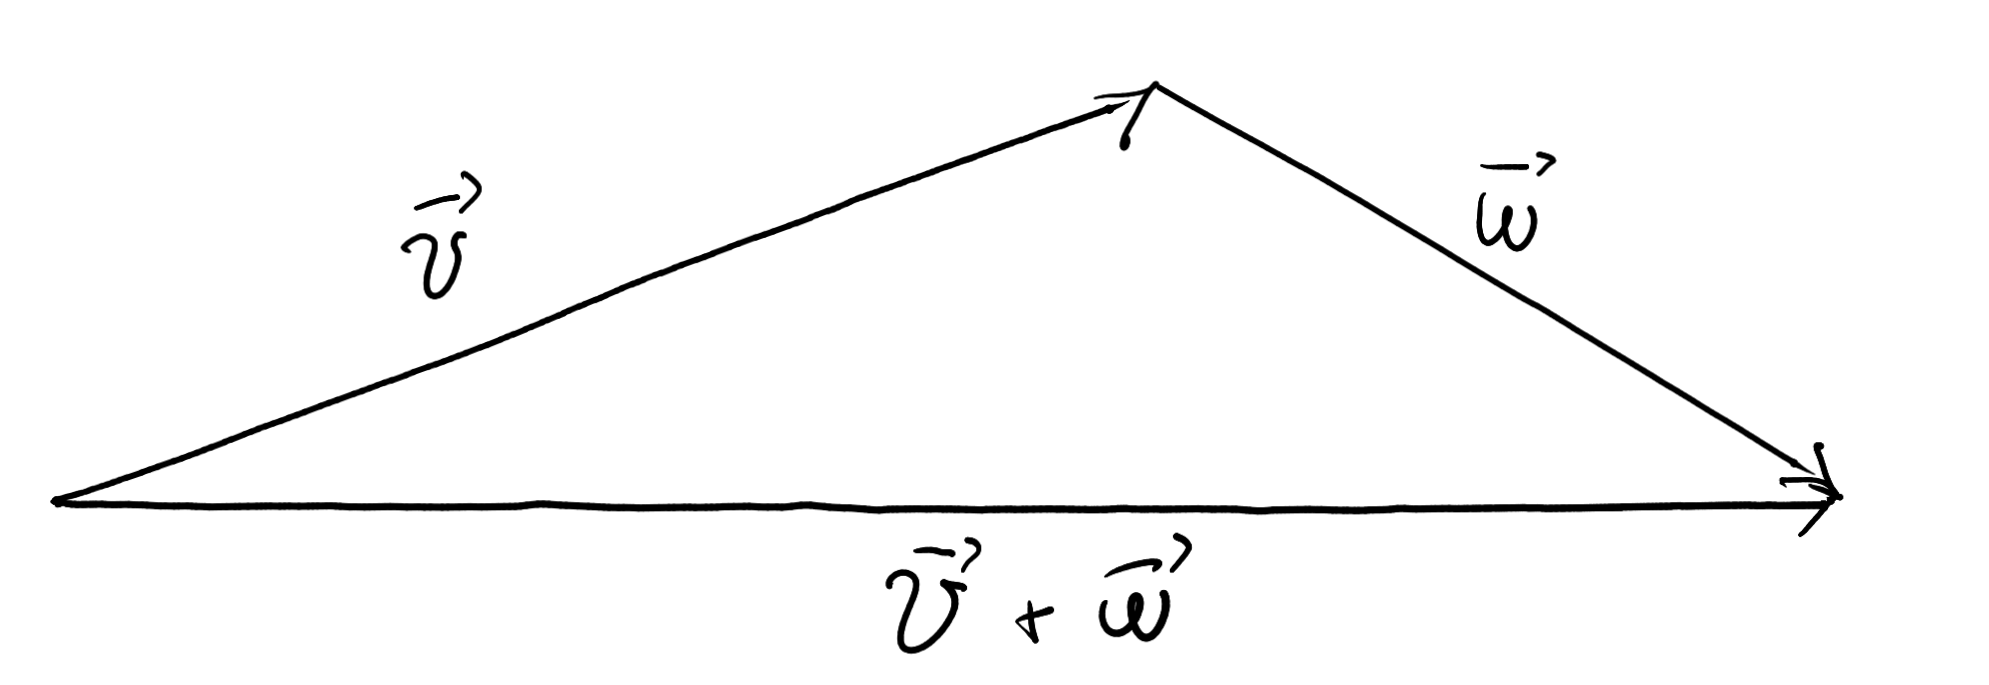
\includegraphics[scale=0.2]{Images/Linear_Algebra-vector-sum1.png}
    \caption{Triangle Law of Vector Addition}
    \label{fig:vector-sum-1}
\end{figure}

Now, let's consider an example of vector addition using two real vectors, $\vec a$ and $\vec b$. The sum of $\vec a$ and $\vec b$ will be:

$$
\vec a = \begin{bmatrix}
    1 \\
    2
\end{bmatrix}
\quad
\vec b = \begin{bmatrix}
    2 \\
    -3
\end{bmatrix}
$$

$$
\vec a + \vec b = \begin{bmatrix}
    a_0 + b_0 \\
    a_1 + b_1
\end{bmatrix} = \begin{bmatrix}
    1 + 2 \\
    2 + (-3)
\end{bmatrix} = \begin{bmatrix}
    3 \\
    -1
\end{bmatrix}
$$

\begin{figure}[h]
    \centering
    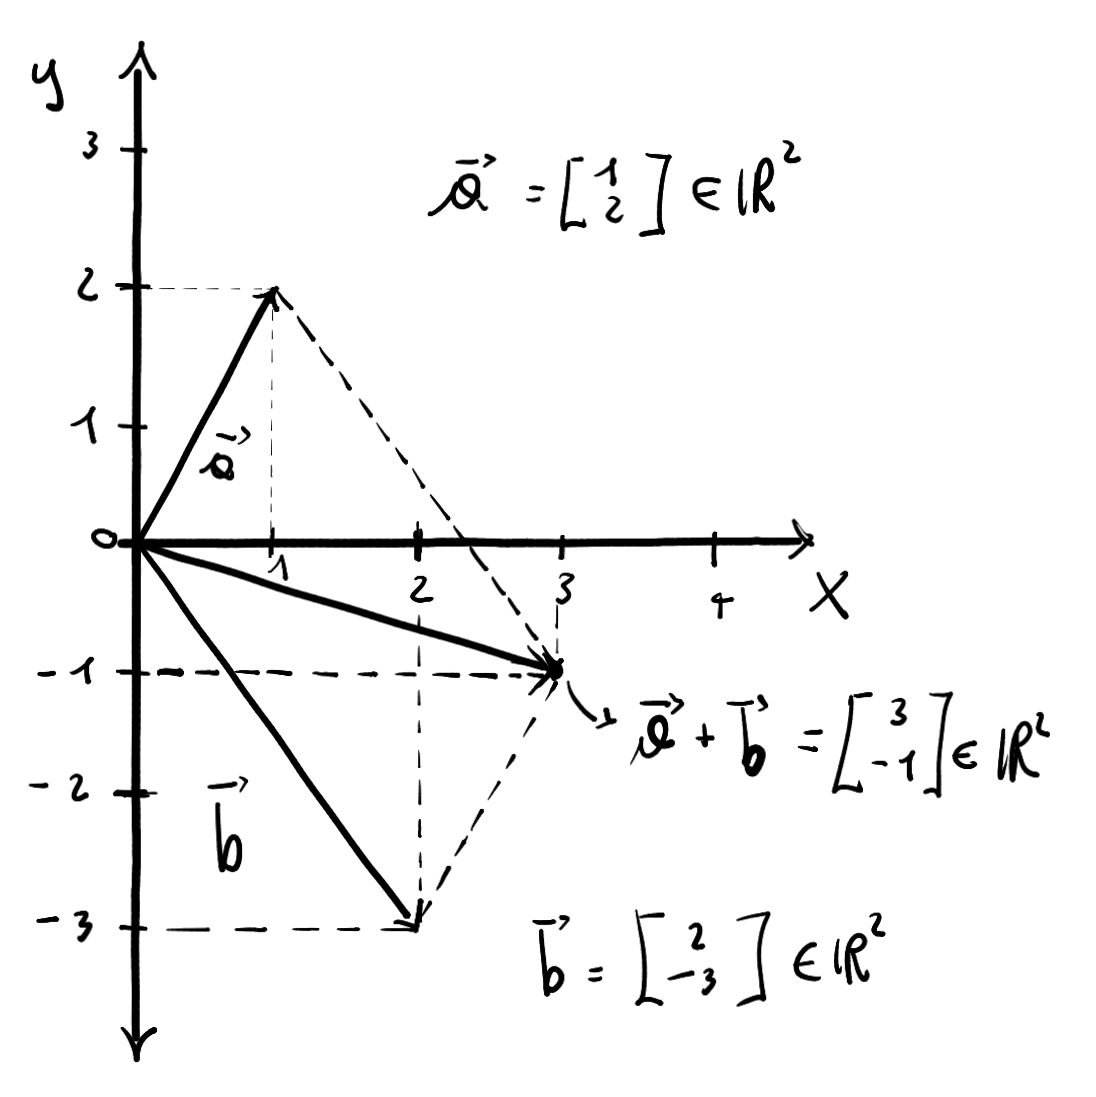
\includegraphics[scale=0.25]{Images/Linear_Algebra-vector-sum2.png}
    \caption{Parallelogram Law of Addition of Vectors}
    \label{fig:vector-sum-2}
\end{figure} 

The Figure \ref{fig:vector-sum-2} shows the vector sum graphically by using the Parallelogram law.

Note that we can sum together only vectors that have the same shape.
\\

The same concept can be applied to matrices, in fact given two matrices 

$$
A_{m,n} = \begin{bmatrix}
    a_{1,1} & a_{1,2} & \dots & a_{1,n} \\
    a_{2,1} & a_{2,2} & \dots & a_{2,n} \\
    \vdots & \vdots & \ddots & \vdots \\
    a_{m,1} & a_{m,2} & \dots & a_{m,n}
\end{bmatrix}, \quad
B_{m,n} = \begin{bmatrix}
    b_{1,1} & b_{1,2} & \dots & b_{1,n} \\
    b_{2,1} & b_{2,2} & \dots & b_{2,n} \\
    \vdots & \vdots & \ddots & \vdots \\
    b_{m,1} & b_{m,2} & \dots & b_{m,n}
\end{bmatrix}
$$

their sum is defined as

\[
A_{m,n} + B_{m,n} =
\begin{bmatrix}
    a_{1,1} + b_{1,1} & \dots & a_{1,n} + b_{1,n} \\
    a_{2,1} + b_{2,1} & \dots & a_{2,n} + b_{2,n} \\
    \vdots & \ddots & \vdots \\
    a_{m,1} + b_{m,1} & \dots & a_{m,n} + b_{m,n}
\end{bmatrix}
=
\begin{bmatrix}
    c_{1,1} & \dots & c_{1,n} \\
    c_{2,1} & \dots & c_{2,n} \\
    \vdots & \ddots & \vdots \\
    c_{m,1} & \dots & c_{m,n}
\end{bmatrix}
= C_{m,n}
\]

or, more mathematically, the generic $c_{i,j}$ of $C_{m,n}$ of new matrices is equal to $a_{i,j} + b_{i,j}$.
Note that we can sum together only matrices that have the same shape.
\\

\subsection{Sum Over Axes}\label{subsection:sum-over-axes}
Now, let's introduce the concept of \textit{sum over axes}.

The \textit{sum over axes} operation plays a crucial role, particularly when dealing with high dimensionality objects. This operation allows us to efficiently contract algebraic objects along specified axes, resulting in a new object with reduced dimension.

Consider a very simple example, imagining having a vector $\vec{v} \in \mathbb{F}^n$ and wanting to perform a \textit{sum over axes} on its (only) axis, i.e., axis 0.

$$
\vec{v} = \begin{bmatrix}
    v_1 \\
    v_2 \\
    \vdots\\
    v_n
\end{bmatrix} \in \mathbb{F}^n \quad \underset{\text{Sum over 0 axis}}{\longrightarrow} = \sum_{i=0}^n v_i
$$

After the sum over the 0 axis of the vector $\vec{v}$, we obtain a scalar belonging to the same field as the vector components. 
\\

So, for example:

\[
\vec{v} = \begin{bmatrix}
    1 \\
    2 \\
    3
\end{bmatrix} \in \mathbb{F}^3 \quad \underset{\text{Sum over 0 axis}}{\longrightarrow} 
\begin{bmatrix}
    1 + 2 + 3
\end{bmatrix} = 6 \in \mathbb{F}
\]

Consider another very simple example, imagining having a matrix $A_{m,n}$ and wanting to perform a \textit{sum over axes} on axis 0.

$$
A_{m,n} = \begin{bmatrix}
    a_{1,1} & a_{1,2} & \dots & a_{1,n} \\
    a_{2,1} & a_{2,2} & \dots & a_{2,n} \\
    \vdots & \vdots & \ddots & \vdots \\
    a_{m,1} & a_{m,2} & \dots & a_{m,n}
\end{bmatrix}  \in \mathbb{F}^{m \times n} \quad \underset{\text{Sum over 0 axis}}{\longrightarrow} A_{1, n}' = 
\begin{bmatrix}
    \sum_{i=0}^m a_{i,1} & \sum_{i=0}^m a_{i,2} & \dots & \sum_{i=0}^m a_{i,n}
\end{bmatrix}
$$

For example:

\[
A_{3,4} = \begin{bmatrix}
    1 & 2 & 3 & -8 \\
    2 & 5 & -1 & 9 \\
    3 & 3 & -7 & -2
\end{bmatrix} \in \mathbb{F}^{3 \times 4} \quad \underset{\text{Sum over 0 axis}}{\longrightarrow} A_{1, 4}' = 
\begin{bmatrix}
    1 & 2 & 3 & -8 \\
    + & + & + & + \\
    2 & 5 & -1 & 9 \\
    + & + & + & + \\
    3 & 3 & -7 & -2
\end{bmatrix}
=
\begin{bmatrix}
    6 & 10 & -5 & -1
\end{bmatrix}
\]

Thus, we have obtained the \textit{sum over axes} on axis 0 of the matrix $A_{5,4}$, obtaining a row vector $A'$ of one dimension and size 4.

Similarly, if we wanted to perform a \textit{sum over axes} on axis 1, we would get

$$
A_{mn} = \begin{bmatrix}
    a_{1,1} & a_{1,2} & \dots & a_{1,n} \\
    a_{2,1} & a_{2,2} & \dots & a_{2,n} \\
    \vdots & \vdots & \ddots & \vdots \\
    a_{m,1} & a_{m,2} & \dots & a_{m,n}
\end{bmatrix} \in \mathbb{F}^{m \times n} \quad \underset{\text{Sum over 1 axis}}{\longrightarrow} A_{m, 1}' =
\begin{bmatrix}
    \sum_{i=0}^n a_{1,i} \\
    \sum_{i=0}^n a_{2,i} \\
    \vdots\\
    \sum_{i=0}^n a_{m,i}
\end{bmatrix}
$$
For example:
\[
A_{3,4} = \begin{bmatrix}
    1 & 2 & 3 & -8 \\
    2 & 5 & -1 & 9 \\
    3 & 3 & -7 & -2
\end{bmatrix} \in \mathbb{F}^{3 \times 4} \quad \underset{\text{Sum over 1 axis}}{\longrightarrow} A_{3, 1}' = 
\begin{bmatrix}
    1 + 2 + 3 - 8 \\
    2 + 5 - 1 + 9 \\
    3 + 3 - 7 - 2
\end{bmatrix}
=
\begin{bmatrix}
    -2 \\
    15 \\
    -3
\end{bmatrix}
\]


\subsection{Multiplication}
When we talk about product, we are, of course, referring to the multiplication between two algebraic objects. When these two objects are scalars, we don't need to consider the issue of dimensionality, as scalars are objects with no dimension, and therefore, their product will inevitably have no dimension. However, as the complexity (and hence, dimension) of the objects we want to multiply increases and differs between the two objects, we need to take into account not only the product itself, but also the dimensional differences involved. In fact, as the shape of the objects increases (and differs), the possible ways of performing their product also increase.

In the following sections, it will become clearer in what ways it is possible to perform the standard product between two objects (scalar, vectors or matrices) and what is the difference with standard product, \textbf{Hadamard} product and \textbf{Kronecker} product.

Esistono molti modi di calcolare il prodotto tra due ogetti algebrici, ma la caratteristica che li accomuna è che tutti i prodotti si basano su due operazioni fondamentali:

\begin{itemize}
    \item Sum over axes.
    \item Moltiplicazione tra scalari.
\end{itemize}

Dove la \textit{sum over axes}, precedentemente introdotta nella sottosezione \ref{subsection:sum-over-axes}, ci permette di eseguire le operazioni di contrazione degli assi necessarie al calcolo del prodotto di due ogetti algebrici.

Mentre il prodotto standard tra scalari è il normale prodotto a cui siamo abituati; definito per due generici elementi $a, b$ del campo $\mathbb{F}$ come:

$$
a \cdot b = c \in \mathbb{F}
$$

Tramite queste due operazioni siamo in grado di eseguire il prodotto di due elementi algebrici di dimensionalità arbitraria.

\subsubsection{Compatibilità tra Assi}

Prima di addentrarci nel calcolo vero e proprio, dobbiamo chiarire anche un altro punto, senza il quale non è possibile eseguire tutte le tipologie di prodotto. Introduciamo quindi il concetto di \textit{compatibilità tra assi}: due assi (dimensioni) si dicono compatibili se e solo se hanno la stessa size (contengono lo stesso numero di elementi). Per asse si intende la dimensione, ad esempio l'asse 0 (l'unico) del vettore $\vec v \in  \mathbb{F}^n$ è la sua dimensione, l'asse del vettore $\vec w \in \mathbb{F}^m$ sono compatibili se e solo se $n = m$. 

Facciamo un altro esempio, siano $A_{3, 2} \in \mathbb{F}^{3 \times 2}$ e $B_{2, 3} \in \mathbb{F}^{2 \times 3}$ due matrici, in questo caso l'asse 0 della matrice $A_{3,2}$ e l'asse 1 della matrice $B_{2, 3}$ sono compatibili, ma anche l'asse 1 della matrice $A_{3,2}$ e l'asse 0 della matrice $B_{2,3}$ lo sono.

Mentre eseguiamo il prodotto di due ogetti algebrici, può essere necessario tenere conto di quali assi sono compatibili, perchè alcuni tipi di prodotto necessitano tale requisito.

\subsubsection{Prodotto}
In generale il prodotto tra due generici ogetti algebrici viene calcolato attraverso una prima fase di scelta degli assi compatibili sui quali effettuare la contrazione, e una seconda fase nella quale si effettua il broadcast sulle dimensioni che non sono state scelte per la contrazione. In generale il risultato è dato da un ogetto che ha per dimensioni tutte le dimensioni "non scelte" in ordine di moltiplicazione. 

In questa sezione ci limiteremo a descrivere le principali metodologie di calcolo del prodotto.
\\
 
L'esempio più semplice (escluso il prodotto tra scalari) è il prodotto di uno scalare per un vettore. In questo caso non si scelgono assi compatibili (perché non ve ne sono) quindi non si effettua la contrazione, ma si passa direttamente alla fase di broadcast dello scalare per ogni componente del vettore. Tale prodotto è definito tra uno scalare $a \in \mathbb F$ e un vettore $\vec v \in \mathbb{F}^n$ e si scrive

$$
a \cdot \vec v = a \cdot \begin{bmatrix}
    v_1\\
    v_2\\
    \vdots\\
    v_n
\end{bmatrix} = \begin{bmatrix}
    a \cdot v_1\\
    a \cdot v_2\\
    \vdots\\
    a \cdot v_n
\end{bmatrix} \in \mathbb F^{n}.
$$

Il risultato è un vettore con la stessa size del vettore moltiplicato. Infatti se prendiamo la shape dello scalare $()$ e la shape del vettore $(n)$ e le mettiamo insieme otteniamo la shape del vettore risultato, che, dato che lo scalare non ha dimensioni, è proprio $(n)$.
\\
\iffalse
Facciamo però un esempio concreto: siano $\vec v = \beg$
\begin{figure}[h]
    \centering
    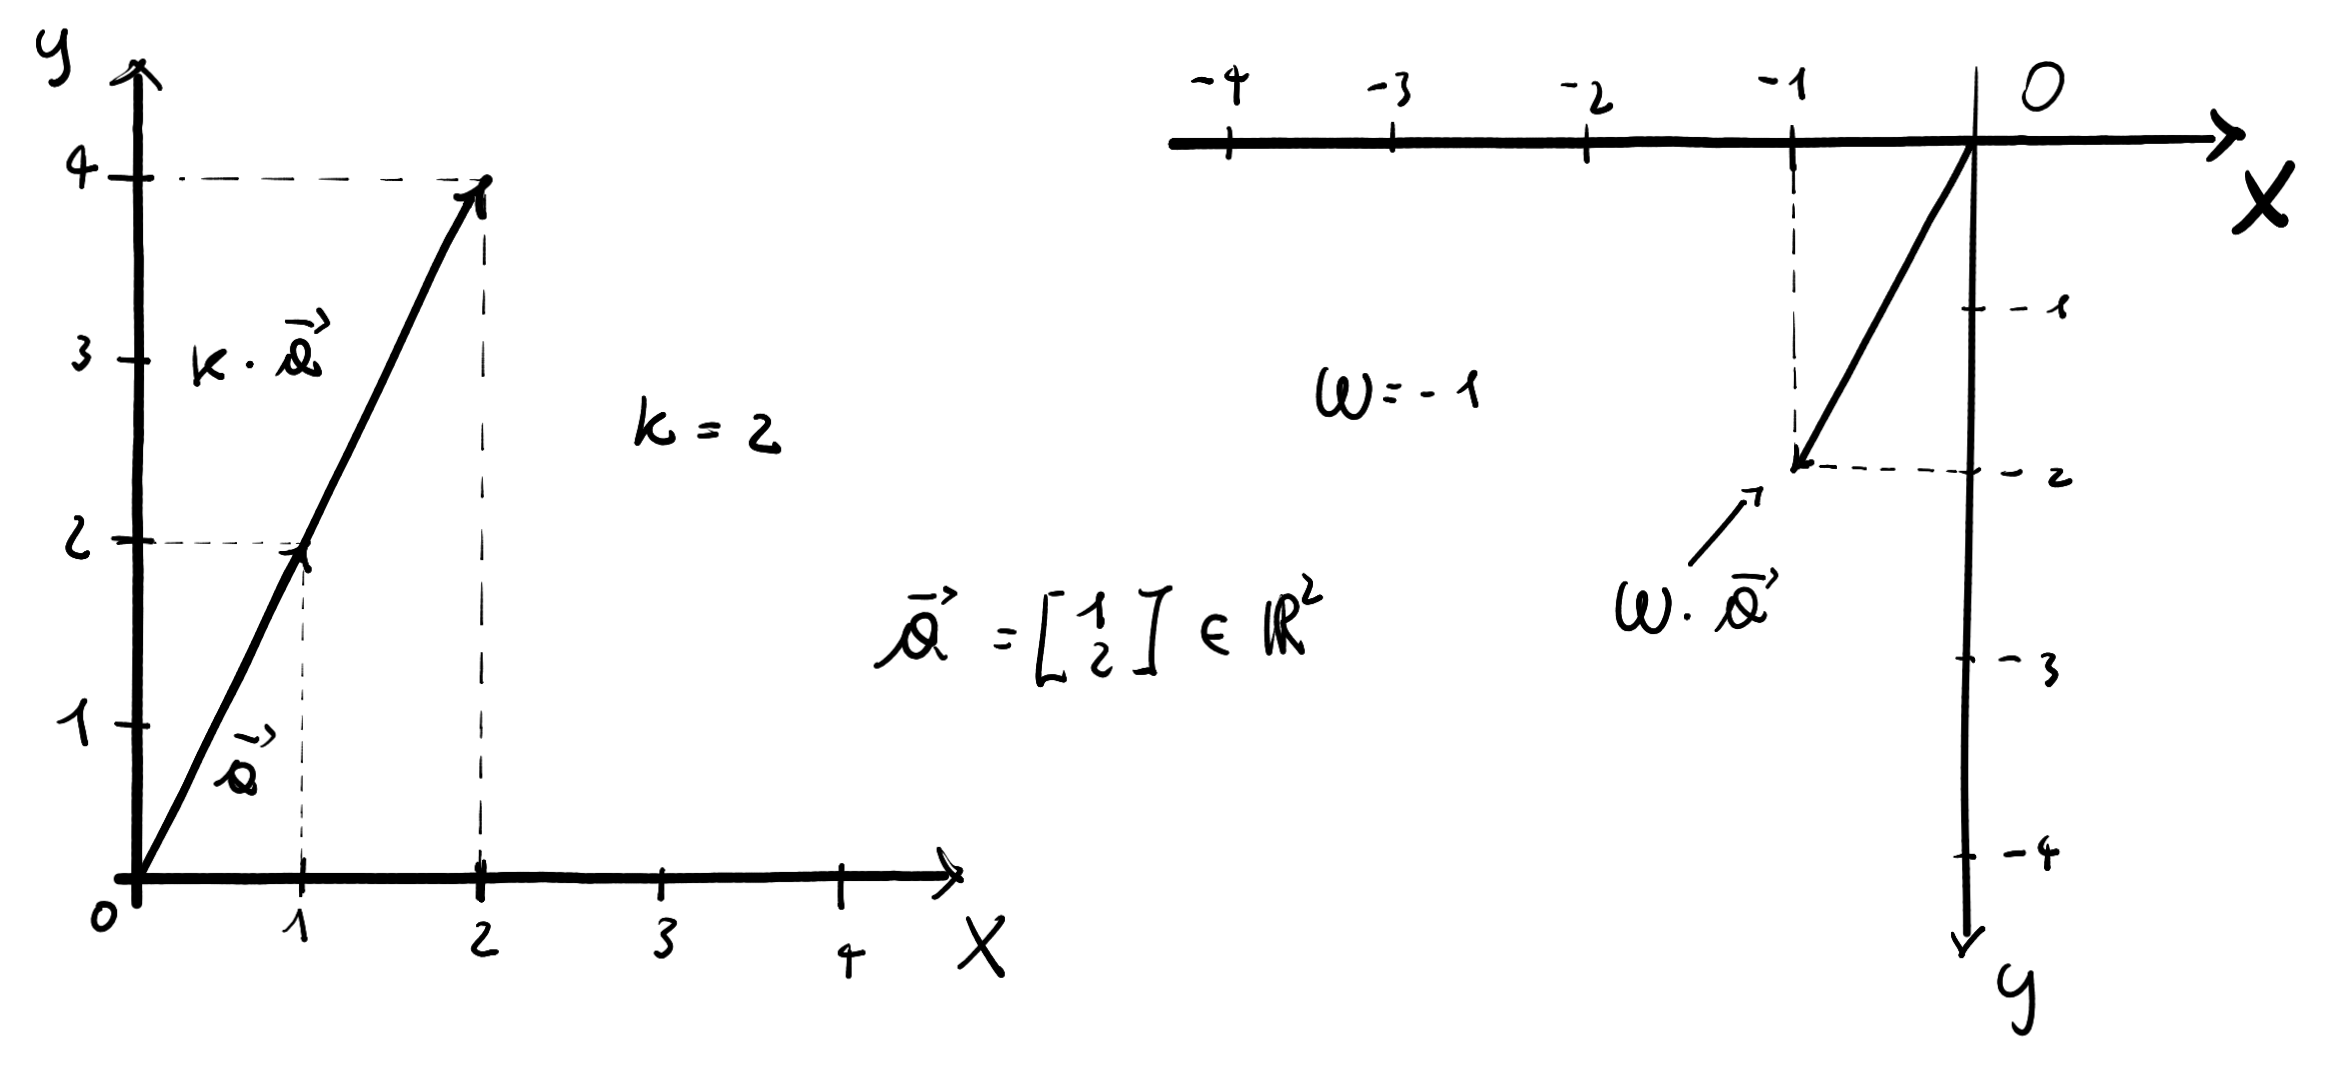
\includegraphics[scale=0.18]{Images/Linear_Algebra-scalar-mul.png}
    \caption{}
    \label{fig:scalar-mul}
\end{figure} 
\fi

% Inserire la definizione di vettore ortogonale

Allo stesso modo, il prodotto tra uno scalare $a \in \mathbb F$ e una matrice $B_{m,n} \in\mathbb F^{m \times n}$ è definito come 

$$
a \cdot B_{m,n} = a \cdot \begin{bmatrix}
    b_{1,1} & \dots & b_{1,n}\\
    b_{2,1} & \dots & b_{1,n}\\
    \vdots  & \ddots & \vdots \\
    b_{m,1} & \dots & b_{m,n}
\end{bmatrix} = \begin{bmatrix}
    a \cdot b_{1,1} & \dots & a \cdot b_{1,n}\\
    a \cdot b_{2,1} & \dots & a \cdot b_{1,n}\\
    \vdots  & \ddots & \vdots \\
    a \cdot b_{m,1} & \dots & a \cdot b_{m,n}
\end{bmatrix} \in \mathbb F^{m \times n}.
$$

Da notare che, come nel caso precedente, lo scalare e la matrice non hanno dimensioni (assi) compatibili, quindi lo scalare viene moltiplicato per tutti i valori della matrice (broadcast). Come risultato finale abbiamo un ogetto che ha per dimensioni le dimensioni dello scalare, che non ne ha, e le dimenisoni della matrice, e quindi $(m,n)$.
\\

Un altro importante prodotto è il prodotto tra vettori. Il \textbf{Dot Product} tra vettori è definito come segue: dati due vettori $\vec v \in  \mathbb{F}^n$ e $\vec w \in \mathbb{F}^n$, il loro prodotto è definito come:

$$
\vec v \cdot \vec w = \begin{bmatrix}
        v_1\\
        \vdots \\
        v_n \\
\end{bmatrix}
    \cdot 
\begin{bmatrix}
        w_1\\
        \vdots \\
        w_n\\
\end{bmatrix} = \sum_{i=0}^n v_i \cdot w_i
$$

Come possimao osservare, scegliendo come assi compatibili: l'asse 0 del primo vettore e l'asse 0 del secondo; possiamo calcolare il prodotto element-wise delle componenti dei due vettori e successivamente, tramite la sum over axes, effettuiamo una contrazione sugli assi compatibili. Come notiamo, non ci sono dimensioni oltre a quelle che abbiamo selezionato, quindi il risultato avrà zero dimensioni e dunque sarà uno scalare.
\\

\`E possibile anche la moltiplicazione tra una matrice ed un vettore. Siano $A_{m,n} \in \mathbb F^{m \times n}$ una matrice e $\vec v \in \mathbb{F}^n$ un vettore. Il loro prodotto è definito come segue:

$$
A_{m,n} \cdot \vec v = \cdot \begin{bmatrix}
    a_{1,1} & \dots & a_{1,n}\\
    a_{2,1} & \dots & a_{1,n}\\
    \vdots  & \ddots & \vdots \\
    a_{m,1} & \dots & a_{m,n}
\end{bmatrix} \cdot \begin{bmatrix}
        v_1\\
        v_2\\
        \vdots \\
        v_n \\
\end{bmatrix} = \begin{bmatrix}
        \sum_{i=0}^n a_{1,i} \cdot v_i\\
        \sum_{i=0}^n a_{2,i} \cdot v_i\\
        \vdots \\
        \sum_{i=0}^n a_{n,i} \cdot v_i \\
\end{bmatrix} \in \mathbb F^{m}
$$

Notiamo che come assi compatibili abbiamo scelto l'unico asse (0) del vettore $\vec v$ e l'asse 1 della matrice $A_{m,n}$, e quindi la contrazione avviene su questa coppia di assi.
Il risultato, come vediamo, ha per dimensioni gli assi non scelti come compatibili nel prodotto, quindi solo l'asse 0 della matrice, che ha come size $m$.

Vediamo ora un esempio con due matrici: siano $A_{m,n} \in \mathbb{F}^{m \times n}$ e $B_{r,s} \in \mathbb{F}^{r \times s}$ due matrici con un asse compatibile (quindi ad esempio $n=r$), il loro prodotto è definito come

$$
A_{m,n} \cdot B_{r,s} = \begin{bmatrix}
    \sum_{i=0}^n a_{1,i} \cdot b_{i,1} & \dots & \sum_{i=0}^n a_{1,i} \cdot b_{i,s}\\
    \vdots & \ddots & \vdots\\
    \sum_{i=0}^n a_{m,i} \cdot b_{i,1} & \dots & \sum_{i=0}^n a_{m,i} \cdot b_{i,s}
\end{bmatrix} = C_{m,s}.
$$

% Proprietà del prodotto tra matrici/vettori/scalari

Abbiamo ottenuto una matrice $C_{m,s}$ che ha lo stesso numero di righe di $A_{m,n}$ e lo stesso numero di colonne di $B_{r, s}$.

Questo è il prodotto matriciale standard più comunemente utilizzato; ve ne sono molti altri che si ottengono facendo una scelta diversa degli assi compatibili su cui fare la contrazione.
\\

% Moltiplicazione a blocchi
%+ Theorem
% Def matrice identità/Inversa

C'è poi un altro particolare prodotto element-wise, che si effettua sugli assi compatibili, ma senza alcuna contrazione. Questo tipo di prodotto si chiama \textbf{Hadamard product} ed è definito solamente per ogetti algebrici con la stessa shape (stesso numero di assi e stassa size per ogni asse).

L'\textbf{Hadamard product} per la generica coppia di vettori $\vec v, \vec w \in \mathbb F^n$ è definito come

$$
\vec v \odot \vec w = \begin{bmatrix}
        v_1\\
        v_2\\
        \vdots \\
        v_n \\
\end{bmatrix} \odot \begin{bmatrix}
        w_1\\
        w_2\\
        \vdots \\
        w_n \\
\end{bmatrix} = \begin{bmatrix}
        v_1 \cdot w_1\\
        v_2 \cdot w_2\\
        \vdots \\
        v_n \cdot w_n\\
\end{bmatrix} \in \mathbb F^{n}.
$$

Analogamente nel caso di due matrici $A_{m,n}, B_{m,n}$ il loro \textbf{Hadamard product} è definito come 

$$
A_{m,n} \odot B_{m,n} = \begin{bmatrix}
    a_{1,1} \cdot b_{1,1} & \dots & a_{1,n} \cdot b_{1,n}\\
    \vdots & \ddots & \vdots\\
    a_{m,1} \cdot b_{m,1} & \dots & a_{m,n} \cdot b_{m,n}
\end{bmatrix} \in \mathbb F^{m \times n}.
$$

In questa sezione sono state illustrate solamente alcune delle tipologie di prodotto che è possibile effettuare nell'algebra lineare. Questo perché si tratta di un testo introduttivo, dove vengono trattati solamente gli aspetti basici dell'algebra lineare che è una materia molto profonda.